%!TEX root = ../dissertation.tex

\chapter{Introduction}
\label{chapter:introduction}
%Chapter 1
%arbitrariness
%principles of comunication -> influence structure?
%timescales
%pragmatic equilibra in the lexicon
%accounts of the length of linguistic elements

%What is the relationship between processes at shorter timescales and language structure?

``Room for cream?'' asked the barista. ``Mm, yes -- just a bit" replied the customer. Mundane linguistic interactions such as this are the building blocks of daily experience. They are individuals making sounds to each other in an effort to coordinate their behavior in the physical world \cite{clark2006social}. These interactions are messy, variable, and highly unconstrained. Indeed it is this variability that gives language its vast expressive power \cite{hockett1960}. Yet, despite this appearance of irregularity, rich patterns in linguistic usage are revealed when we aggregate across instances of language use both within and across languages. At the level of syntax, for example, there is a strong bias in English to put subjects before verbs and, across languages, this pattern is attested more often than would be expected by chance alone  \cite{dryer2005order}. These types of probabilistic regularities exist at every level of linguistic structure---from phonology, to semantics, syntax, and discourse---and researchers from a variety of disciplines have taken as their project the goal of characterizing these regularities.

%Where does linguistic structure come from? \citeA[2010]{christiansen2008} propose a compelling theory. They argue that  multiple cognitive constraints dynamically influence language evolution. They suggest four constraints: the representational format of thought, properties of the percepto-motor system, learning and processing constraints, and constraints that result from reasoning about others' intentions ({\it pragmatic} constraints). Their argument is that these constraints  influence  language at the moment of use, but over time, these biases become instantiated in the structure of language. 

In this dissertation, I contribute to this effort with a focus on understanding on how language use shapes language structure. I am particularly interested in how  aspects of the environment of linguistic interaction, including the cognitive system itself, can over time influence the emergence of a regularity in the linguistic system. As a conceptual framework for exploring these dynamics, I will appeal to the notion of a {\it timescale}. A timescale is a unit of time over which significant changes in state occur. For example, the timescale of dinner is about an hour, where the significant changes in state are walking to the restaurant, sitting down, ordering food, eating the meal, then dessert, etc. In contrast, the timescale of gaining weight occurs over weeks, where the significant changes in state correspond to appreciable weight changes. Critically, the length of the timescales is determined by the change of interest. 

\begin{figure}
\begin{center} 
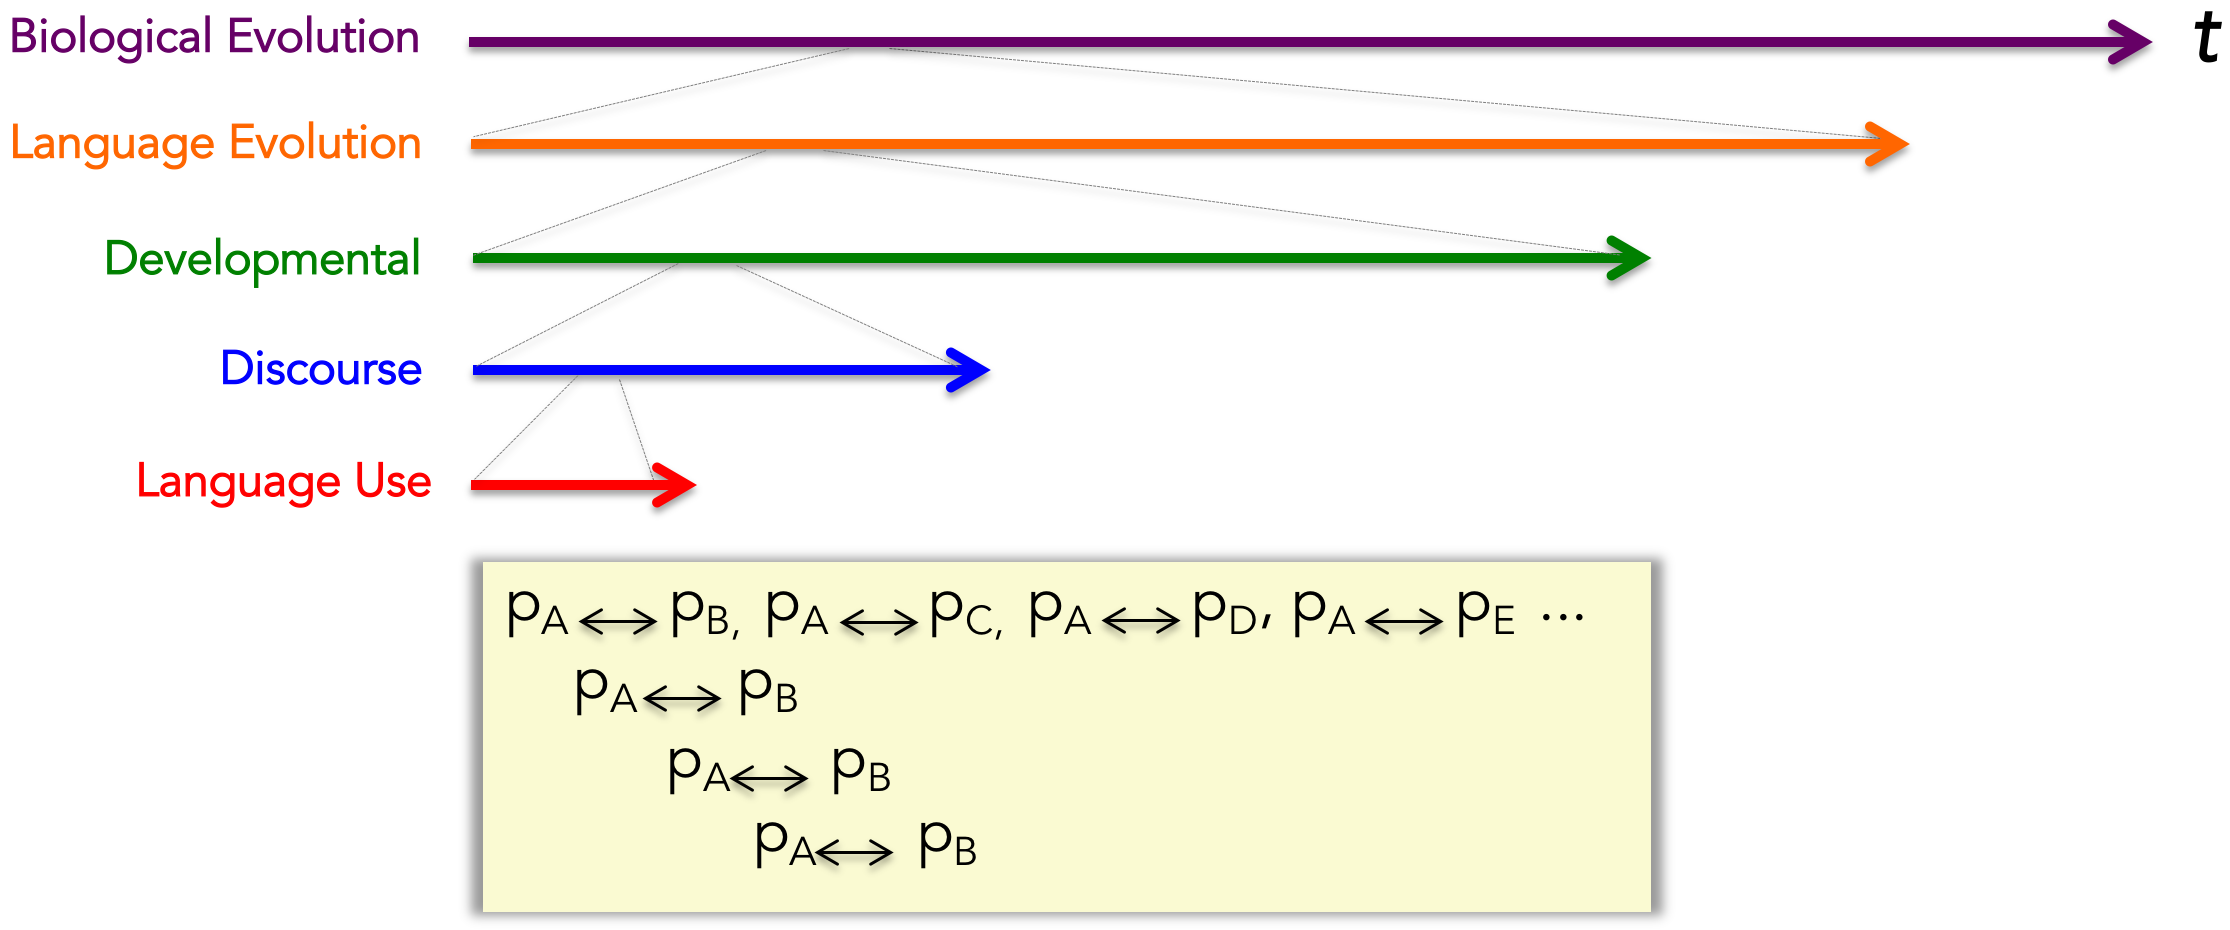
\includegraphics[width=6in]{figs/timescales2}
\caption{The five linguistic timescales. Each timescale is nested within a slice of longer timescales. The claim is that the dynamics between adjacent timescales (e.g., language use and discourse) lead to changes over time in longer timescales. The developmental timescale is characterized by a particular person from a particular generation, $p_A$, interacting with a series of people over the lifespan. Repeated interactions with the same person, $p_B$, characterize the discourse timescale.}
\label{fig:timescales}
\end{center} 
\end{figure}



In the case of language, the central  hypothesis is that there are pressures at  short timescales that over long periods of time lead to changes in the structure of language. More specifically,  there are five timescales over which significant linguistic changes may occur (presented in Figure \ref{fig:timescales}). The first is the {\it language use timescale}. The language use timescale takes places over the course of the moments of communicative interaction, and corresponds to the processes  that the emerge as a consequence of reasoning about the intention of one's interlocutor (pragmatic pressures), and in-the-moment pressures of the cognitive system (e.g., memory constraints).  The {\it discourse timescale} is a slightly longer timescale. The discourse timescale corresponds to repeated interactions with the same person; a series of pragmatic interactions. The third is the {\it developmental timescale}. The developmental timescale corresponds to the lifetime of an individual. It is composed of many interactions (on the language use timescale), some of which with the same people (on the discourse timescale).  Many people interacting over their lifetimes lead to change at the {\it language evolution timescale}. This is the timescale over which significant changes in language structure  occur. Finally, at the longest timescale, is the {\it biological evolution timescale}. All of the dynamics at lower timescales occur within a small slice in evolutionary time. I will not have much to say about this timescale; its main significance is to situate the present claims with respect to claims about the innateness of language. Following \citeA{christiansen2008}, the suggestion is that there are aspects of language that are innate and constrain the dynamics of shorter timescales. Importantly, however, there are also  dynamics that take place at  shorter timescales, and these dynamics are the focus here.


% The alternative hypothesis is that these regularities are the product of innate endowment.
The proposal, then, is that there are dynamics between adjacent timescales, and that, over time, these dynamics lead to change on longer timescales.  Importantly, the character and phenomena of the dynamics between each pair of timescales are different. For example,  the dynamics between discourse and developmental timescales are reflected in cognitive changes in the mind of a particular speaker. In contrast, the dynamics between language evolution and biological evolution timescales are reflected in genetic changes in linguistic abilities. In Chapter 2, we review evidence suggesting a causal link between processes at the language use timescale, particularly pragmatic pressures, and those at the language evolution timescale.

It is worth reflecting on the historical relationship between processes at shorter timescales and language structure. Across many schools of linguistics, theorists have made a theoretical cut between language use and language structure: {\it parole} vs.\  {\it langue}  \cite{saussure},  {\it token}  vs.\  {\it type}  \cite{peirce}, and  {\it performance}  vs.\  {\it competence}  \cite{chomsky1965aspects}. These theorists  have different views on the ontological status of structure---Saussure suggests it is a social fact, while Chomsky argues it is fundamentally a cognitive phenomenon---but they nonetheless agree that there is some sort of invariance in language and it should be the focus of study. Language use has often been seen as an irregular, variant, and epiphenomenal to the true subject of study: structure. However, a number of more recent movements have begun to focus on language use. \nocite{labov197213} Labov's (1972) work was an important challenge to exclusionary focus on abstract structure. His work revealed systematicity in the variation of phonology as function of social variables, suggesting that ``messy" language use was governed by regularities and could therefore be studied scientifically. The study of pragmatics, more generally, can be seen as a step to find regularity in language use. 

A number of theorists have suggested a causal link between use and linguistic structure. One of the earliest proposals of this idea was \citeA{whorf1956language} who argued that habitual patterns of talking in particular ways (what he called ``fashions of speaking") lead over time to different conceptualizations of the world.\footnote{This is an important nuance to claims about linguistic relativity that is often over-looked: It is not {\it that} a language has a label for a concept that matters,  but rather the presence of that label in conjunction with a developmental history of using that label.} Grammar is a case where this view as been particularly well articulated, under the heading of {\it Emergent Grammar} \cite{hopper1987emergent}: 

\begin{quote} The notion of Emergent Grammar is meant to suggest that structure, or regularity, comes out of discourse and is shaped by discourse as much as it shapes discourse in an on-going process. [...] Structure, then, in this view is not an overarching set of abstract principles, but more a question of a spreading of systematicity from individual words, phrases and small sets. (p. 142)
\end{quote}
More recently, cognitive psychologists have begun to formally model these dynamics. In this tradition, \citeA{bybee2005alternatives} write: ``Properties of formal structure [...] are facts about the structure that are to be explained as arising from the cumulative impact of the processes that shape each language, as it adapts through the process of language use" (p. 406). They argue for the value of a connectionist framework in capturing these dynamics. Also within a  connectionist framework, \citeA{mcmurray2012} highlight the relevance of different timescales in capturing the phenomenon of children's word learning across the developmental timescale. Perhaps the broadest framing of these dynamics has been by \citeA{christiansen2008} who propose a mechanism closely aligned with the present argument.

The focus of this dissertation is on one aspect of language structure,  a {\it complexity bias}, as a case study in understanding a potential causal link between language use and language structure. We define a complexity bias in the following way:
\begin{quote}
{\it Complexity Bias}: A probabilistic bias for languages to assign conceptually complex meanings to long words and conceptually simple meanings  to short words.
\end{quote}
To be concrete, this bias predicts that a meaning with many conceptual parts, like \textsc{computer}, will be encoded linguistically with a longer label than a meaning with fewer conceptual parts, like  \textsc{hat}. The study of this particular aspect of linguistic structure, a complexity bias, is motivated by several different cognitive and communicative pressures at the language use timescale. The first is a bias to map meanings onto perceptually similar linguistic forms; that is, a bias for iconicity. There is a large body of evidence suggesting that aspects of language  contain iconic elements \cite<see>[for review]{schmidtke2014phonological}. In addition, several theories of communication---Information Theory  \cite{shannon1948} and Horn's theory of communication (1984)---predict a tradeoff between length and conceptually complexity within language systems. Briefly, these two theories suggest that communication systems can maximize information transfer and minimize effort by mapping conceptually complex meanings to long words. We outline this prediction in more detail in the Introduction to Chapter 2.


The plan of this dissertation is as follows. In Chapter 2, we begin by examining whether languages do indeed have a complexity bias, and whether speakers have a complexity bias when faced with novel words and meanings. In this chapter, we appeal to a largely intuitive notion of conceptual complexity, assuming that objects with more physical `parts' are more conceptually complex. Across a series of ten studies we find evidence  that both languages and individual speakers have a complexity bias. In Chapter 3, we turn to the question of what conceptual complexity is more directly. Across seven studies, we explore a variety of hypotheses about the nature of conceptual complexity, ranging from the number of conceptual features a meaning has to the frequency of the object in the world. In Chapter 4, we ask how a complexity bias might come to be in the natural language over the course of language evolution. We appeal to evidence from four different studies and conclude that most evidence favors the possibility that the regularity derived from a cognitive bias for iconicity.  Finally, Chapter 5 takes a broader view on the question of how pressures of language use might shape language structure. Here we ask how a wide range of factors, across a range of timescales, might over time influence linguistic structure. 



